% ============================================================================
%  Master Derivations — Pipeline of Coherence
%  All Formulas, Derivations, and Theorems from the Kernel Repository
%
%  Framed by the critical complex equilibrium:
%      µ = e^{i3π/4} = (-1+i)/√2
%  — the unique balanced eigenvalue on the unit circle with
%    negative real part and positive imaginary part.
% ============================================================================

\documentclass[12pt,a4paper]{article}

%% ── Packages ─────────────────────────────────────────────────────────────────
\usepackage[T1]{fontenc}
\usepackage[utf8]{inputenc}
\usepackage{lmodern}
\usepackage{amsmath,amssymb,amsthm}
\usepackage{mathtools}
\usepackage{bm}
\usepackage{booktabs}
\usepackage{array}
\usepackage{pgfplots}
\pgfplotsset{compat=1.18}
\usepackage{xcolor}
\usepackage{hyperref}
\usepackage{geometry}
\usepackage{microtype}
\usepackage{setspace}
\usepackage{mdframed}
\usepackage{tcolorbox}
\tcbuselibrary{skins,breakable}

\geometry{margin=2.5cm}
\onehalfspacing

%% ── Theorem environments ─────────────────────────────────────────────────────
\theoremstyle{plain}
\newtheorem{theorem}{Theorem}[section]
\newtheorem{lemma}[theorem]{Lemma}
\newtheorem{corollary}[theorem]{Corollary}
\newtheorem{proposition}[theorem]{Proposition}

\theoremstyle{definition}
\newtheorem{definition}[theorem]{Definition}
\newtheorem{example}[theorem]{Example}

\theoremstyle{remark}
\newtheorem{remark}[theorem]{Remark}
\newtheorem{conjecture}[theorem]{Conjecture}

%% ── Highlighted box for the critical equilibrium ─────────────────────────────
\tcbset{
  equilibrium/.style={
    enhanced, breakable,
    colback=gray!8, colframe=black!70,
    boxrule=1.2pt, arc=4pt,
    title style={font=\bfseries\large},
    fonttitle=\bfseries\large,
  }
}

%% ── Math macros ──────────────────────────────────────────────────────────────
\newcommand{\C}{\mathbb{C}}
\newcommand{\R}{\mathbb{R}}
\newcommand{\Z}{\mathbb{Z}}
\newcommand{\ket}[1]{\lvert #1 \rangle}
\newcommand{\bra}[1]{\langle #1 \rvert}
\newcommand{\abs}[1]{\lvert #1 \rvert}
\newcommand{\norm}[1]{\lVert #1 \rVert}
\newcommand{\floor}[1]{\lfloor #1 \rfloor}
\newcommand{\ceil}[1]{\lceil #1 \rceil}
\newcommand{\dS}{\delta_S}        % silver ratio 1+√2
\newcommand{\Cr}{C(r)}            % coherence function
\newcommand{\Rr}{R(r)}            % palindrome residual
\newcommand{\Geff}{G_{\mathrm{eff}}}
\newcommand{\Reff}{R_{\mathrm{eff}}}
\newcommand{\mubal}{\mu}          % balanced eigenvalue e^{i3π/4}

%% ── Part numbering (A, B, C …) ───────────────────────────────────────────────
\renewcommand{\thepart}{\Alph{part}}

%% ── Title ────────────────────────────────────────────────────────────────────
\title{%
  \textbf{Master Derivations — Pipeline of Coherence}\\[0.5em]
  \large All Formulas, Derivations, and Theorems\\
  from the Kernel Repository\\[0.4em]
  \normalsize Framed by the Critical Complex Equilibrium
  $\mu = e^{i3\pi/4}$
}
\author{%
  Kernel Repository\\
  \href{https://github.com/beanapologist/Kernel}{github.com/beanapologist/Kernel}
}
\date{February 2026}

% ============================================================================
\begin{document}
\maketitle
\tableofcontents
\newpage

%% ════════════════════════════════════════════════════════════════════════════
%% OPENING: THE CRITICAL COMPLEX EQUILIBRIUM
%% ════════════════════════════════════════════════════════════════════════════

\begin{tcolorbox}[equilibrium, title={Critical Complex Equilibrium}]
\begin{equation}
\boxed{
  \mu \;=\; e^{i3\pi/4}
      \;=\; \frac{-1 + i}{\sqrt{2}}
      \;=\; -\frac{1}{\sqrt{2}} + \frac{i}{\sqrt{2}},
      \qquad \abs{\mu} = 1,\quad \arg(\mu) = \tfrac{3\pi}{4}.
}
\label{eq:mu-def}
\end{equation}
\vspace{2pt}
$\mu$ is the unique eighth root of unity lying in the \textbf{second quadrant}
of $\C$: negative real part $-1/\sqrt{2}$ and positive imaginary part
$+1/\sqrt{2}$.  It is the balanced eigenvalue at the heart of all constructions
in this document.  The entire theory emanates from $\mu$ and returns to it:
\[
  \mu^8 = 1,\qquad \gcd(3,8)=1 \;\Rightarrow\; \{1,\mu,\mu^2,\ldots,\mu^7\}
  \text{ partitions the unit circle into 8 equal slices of }45^\circ.
\]
\end{tcolorbox}

\bigskip

This document collects, in logical order, \emph{every} formula, derivation,
and theorem from the Kernel repository.  The exposition begins with the
fundamental constants and eigenvalue structure, builds the coherence framework,
derives the palindrome precession geometry, proves the $\Theta(\sqrt{n})$
complexity bound, presents the Ohm--Coherence duality, and concludes by
returning to the critical equilibrium $\mu$.

%% ════════════════════════════════════════════════════════════════════════════
\part{Proven Identities}
\label{part:proven}
%% ════════════════════════════════════════════════════════════════════════════

%% ════════════════════════════════════════════════════════════════════════════
\section{Fundamental Constants}
\label{sec:constants}
%% ════════════════════════════════════════════════════════════════════════════

\subsection{Theorem~3 — Critical Constant \texorpdfstring{$\eta = 1/\sqrt{2}$}{eta}}

\begin{theorem}[Critical constant]\label{thm:3}
  The equation $2\lambda^2 = 1$ has a unique positive root
  \begin{equation}
    \eta \;=\; \frac{1}{\sqrt{2}} \;=\; \frac{\sqrt{2}}{2}
         \;\approx\; 0.7071067811865475.
    \label{eq:eta}
  \end{equation}
  This value satisfies $\eta^2 + \eta^2 = 1$ exactly, making it the unique
  amplitude for a balanced two-component state
  $(\abs{\alpha},\abs{\beta}) = (\eta,\eta)$ with unit norm.
\end{theorem}

\begin{proof}
  Substituting $\lambda = 1/\sqrt{2}$ gives $2(1/\sqrt{2})^2 = 2\cdot\tfrac{1}{2} = 1$.
  Uniqueness follows since $f(\lambda)=2\lambda^2$ is strictly increasing for
  $\lambda>0$. \qed
\end{proof}

\subsection{Proposition~4 — Silver Conservation}

\begin{proposition}[Silver conservation]\label{prop:4}
  Define the \emph{silver ratio} $\dS = 1+\sqrt{2}$ and its conjugate
  $\dS^{-1} = \sqrt{2}-1$.  Then:
  \begin{align}
    \dS \cdot (\sqrt{2}-1) &= 1,  \label{eq:silver-prod}\\
    \dS^2 &= 2\dS + 1,            \label{eq:silver-sq}\\
    1/\dS &= \sqrt{2}-1.          \label{eq:silver-inv}
  \end{align}
\end{proposition}

\begin{proof}
  \eqref{eq:silver-prod}: $(1+\sqrt{2})(\sqrt{2}-1) = \sqrt{2}-1+2-\sqrt{2} = 1$.
  \eqref{eq:silver-sq}: $(1+\sqrt{2})^2 = 1+2\sqrt{2}+2 = 3+2\sqrt{2}$;
  $2(1+\sqrt{2})+1 = 3+2\sqrt{2}$. \quad
  \eqref{eq:silver-inv}: follows from \eqref{eq:silver-prod}. \qed
\end{proof}

\noindent
\textbf{Numerical values:}
\[
  \dS \approx 2.41421356237,\qquad
  \dS^{-1} \approx 0.41421356237,\qquad
  \dS \cdot \dS^{-1} = 1.
\]

%% ════════════════════════════════════════════════════════════════════════════
\section{The Critical Eigenvalue and Its Orbit}
\label{sec:eigenvalue}
%% ════════════════════════════════════════════════════════════════════════════

\subsection{Section~2 — Eigenvalue \texorpdfstring{$\mu = e^{i3\pi/4}$}{mu}}

\begin{definition}[Balanced eigenvalue]\label{def:mu}
  The \emph{balanced eigenvalue} is
  \begin{equation}
    \mu \;=\; e^{i3\pi/4}
        \;=\; \cos\!\tfrac{3\pi}{4} + i\sin\!\tfrac{3\pi}{4}
        \;=\; -\tfrac{1}{\sqrt{2}} + \tfrac{i}{\sqrt{2}}
        \;=\; \eta(-1+i),
    \label{eq:mu}
  \end{equation}
  where $\eta = 1/\sqrt{2}$ (Theorem~\ref{thm:3}).
  It lies on the unit circle in the second quadrant.
\end{definition}

\begin{proposition}\label{prop:mu-props}
  The eigenvalue $\mu$ satisfies:
  \begin{align}
    \abs{\mu} &= 1, \label{eq:mu-norm}\\
    \arg(\mu) &= \tfrac{3\pi}{4}, \label{eq:mu-arg}\\
    \mu^8 &= 1 \quad(\text{primitive 8th root of unity}), \label{eq:mu-8}\\
    \gcd(3,8) &= 1 \;\Rightarrow\; \{1,\mu,\mu^2,\ldots,\mu^7\}
               \text{ are all distinct.} \label{eq:mu-distinct}
  \end{align}
\end{proposition}

\begin{proof}
  \eqref{eq:mu-norm}: $\abs{\mu}^2 = \eta^2+\eta^2 = 1$.
  \eqref{eq:mu-arg}: by definition.
  \eqref{eq:mu-8}: $(e^{i3\pi/4})^8 = e^{i6\pi} = 1$.
  \eqref{eq:mu-distinct}: since $\gcd(3,8)=1$, multiplying by $\mu$ permutes
  all 8 residues of $\Z/8\Z$. \qed
\end{proof}

\subsection{Section~3 — Rotation Matrix \texorpdfstring{$R(3\pi/4)$}{R(3pi/4)}}

Multiplication by $\mu$ on $\C$ corresponds to the real rotation matrix
\begin{equation}
  R\!\left(\tfrac{3\pi}{4}\right)
  =
  \begin{pmatrix}
    \cos\tfrac{3\pi}{4} & -\sin\tfrac{3\pi}{4}\\[4pt]
    \sin\tfrac{3\pi}{4} &  \cos\tfrac{3\pi}{4}
  \end{pmatrix}
  =
  \begin{pmatrix} -\eta & -\eta \\ \eta & -\eta \end{pmatrix},
  \label{eq:rot-matrix}
\end{equation}
acting on $\mathbf{v} = (x,y)^\top \in \R^2$.

\begin{proposition}[Rotation matrix properties]\label{prop:rot}
  \begin{align}
    \det R &= (-\eta)(-\eta) - (-\eta)(\eta) = \eta^2+\eta^2 = 1,
      \label{eq:det-R}\\
    R^\top R &= I_2 \quad(\text{orthogonality}),
      \label{eq:orth-R}\\
    R^8 &= I_2 \quad(\text{8-step periodicity}).
      \label{eq:R8}
  \end{align}
\end{proposition}

\begin{proof}
  \eqref{eq:det-R}: direct computation.
  \eqref{eq:orth-R}: $R$ is an orthogonal matrix ($\det R = 1$, real, and
  $R^\top = R^{-1}$).
  \eqref{eq:R8}: follows from $\mu^8 = 1$. \qed
\end{proof}

The eight orbit points of $\mu$ at angles $3\pi k/4$, $k=0,\ldots,7$, are:
\begin{equation}
  \{1,\, \mu,\, i,\, -\bar\mu,\, -1,\, -\mu,\, -i,\, \bar\mu\}
  = \bigl\{e^{i3\pi k/4} : k=0,\ldots,7\bigr\},
  \label{eq:orbit8}
\end{equation}
uniformly spaced at $45^\circ$ intervals on the unit circle.

%% ════════════════════════════════════════════════════════════════════════════
\section{Quantum State and Balance}
\label{sec:state}
%% ════════════════════════════════════════════════════════════════════════════

\subsection{Theorem~8 — Canonical Coherent State}

\begin{theorem}[Canonical coherent state]\label{thm:8}
  The \emph{canonical coherent state} is
  \begin{equation}
    \ket{\psi} = \alpha\ket{0} + \beta\ket{1},\qquad
    \alpha = \frac{1}{\sqrt{2}},\quad
    \beta  = \frac{e^{i3\pi/4}}{\sqrt{2}} = \frac{-1+i}{2},
    \label{eq:canonical}
  \end{equation}
  with $\abs{\alpha}^2+\abs{\beta}^2=1$.  In component form,
  $\abs{\alpha}=\abs{\beta}=\eta=1/\sqrt{2}$.
\end{theorem}

\begin{proof}
  $\abs{\alpha}^2 = \eta^2 = 1/2$.
  $\abs{\beta}^2 = \abs{(-1+i)/2}^2 = (1+1)/4 = 1/2$.
  Sum equals 1. \qed
\end{proof}

\begin{definition}[Radius parameter]\label{def:r}
  For any normalised state $(\alpha,\beta)$ with $\abs{\alpha}>0$, the
  \emph{radius parameter} is
  \begin{equation}
    r = \frac{\abs{\beta}}{\abs{\alpha}}.
    \label{eq:radius}
  \end{equation}
  At the canonical state, $r=1$.
\end{definition}

\subsection{Theorem~9 — Balance $\leftrightarrow$ Maximum Coherence}

\begin{theorem}[Balance-coherence equivalence]\label{thm:9}
  For a normalised state $(\alpha,\beta)$ with $r=\abs{\beta}/\abs{\alpha}$:
  \begin{equation}
    \abs{\alpha}=\abs{\beta}=\frac{1}{\sqrt{2}}
    \;\;\Longleftrightarrow\;\;
    C_{\ell^1} = 2\abs{\alpha}\abs{\beta} = 1.
    \label{eq:balance-coherence}
  \end{equation}
  Equivalently, $r=1$ is the \emph{unique} maximiser of $C_{\ell^1}$.
\end{theorem}

\begin{proof}
  $C_{\ell^1} = 2\abs{\alpha}\abs{\beta}$.  By AM-GM,
  $2\abs{\alpha}\abs{\beta} \le \abs{\alpha}^2+\abs{\beta}^2 = 1$,
  with equality iff $\abs{\alpha}=\abs{\beta}=1/\sqrt{2}$, i.e.\ $r=1$. \qed
\end{proof}

%% ════════════════════════════════════════════════════════════════════════════
\section{Coherence, Residual, and Lyapunov Functions}
\label{sec:coherence}
%% ════════════════════════════════════════════════════════════════════════════

\subsection{Theorem~11 — Coherence Function}

\begin{theorem}[Coherence function]\label{thm:11}
  The $\ell^1$ coherence as a function of $r>0$ is
  \begin{equation}
    C(r) \;=\; \frac{2r}{1+r^2}.
    \label{eq:coherence}
  \end{equation}
  Properties:
  \begin{enumerate}
    \item $C(1) = 1$ (global maximum).
    \item $C(r) = C(1/r)$ for all $r>0$ (symmetric about $r=1$).
    \item $\frac{dC}{dr}\big|_{r=1} = 0$,\quad
          $\frac{d^2C}{dr^2}\big|_{r=1} = -1 < 0$ (strict local maximum).
    \item $0 < C(r) < 1$ for all $r\ne 1$.
  \end{enumerate}
\end{theorem}

\begin{proof}
  Writing $C(r)=2r/(1+r^2)$:
  \begin{itemize}
    \item $C(1) = 2/2 = 1$.
    \item $C(1/r) = (2/r)/(1+1/r^2) = (2/r)\cdot r^2/(r^2+1) = 2r/(1+r^2) = C(r)$.
    \item $C'(r) = [2(1+r^2) - 2r\cdot 2r]/(1+r^2)^2 = 2(1-r^2)/(1+r^2)^2$;
          at $r=1$: $C'(1)=0$.
    \item $C''(r) = -4r(3-r^2)/(1+r^2)^3$; at $r=1$: $C''(1)=-4/4=-1<0$. \qed
  \end{itemize}
\end{proof}

\subsection{Theorem~12 — Palindrome Residual}

\begin{theorem}[Palindrome residual]\label{thm:12}
  Define
  \begin{equation}
    R(r) \;=\; \frac{1}{\dS}\!\left(r - \frac{1}{r}\right),
    \qquad r>0,
    \label{eq:palindrome-residual}
  \end{equation}
  where $\dS = 1+\sqrt{2}$ (Proposition~\ref{prop:4}).  Then:
  \begin{enumerate}
    \item $R(r) = 0 \;\Leftrightarrow\; r = 1$.
    \item $R(r) > 0$ for all $r > 1$.
    \item $R(r) < 0$ for all $0 < r < 1$.
    \item $R$ is strictly monotone increasing on $(0,\infty)$.
  \end{enumerate}
\end{theorem}

\begin{proof}
  $R(r) = 0$ iff $r = 1/r$ iff $r=1$ (since $r>0$).
  $R'(r) = (1/\dS)(1 + 1/r^2) > 0$ for all $r>0$ (strictly increasing). \qed
\end{proof}

\subsection{Theorem~14 — Lyapunov--Coherence (Ohm--Coherence) Duality}

\begin{theorem}[Lyapunov--Coherence Duality]\label{thm:14}
  Let $\lambda = \ln r$ (the \emph{Lyapunov exponent} of the state).  Then:
  \begin{equation}
    C(r) \;=\; \operatorname{sech}(\lambda)
         \;=\; \frac{1}{\cosh(\lambda)},
    \label{eq:sech-duality}
  \end{equation}
  with the identification
  \begin{equation}
    \Geff(\lambda) = \operatorname{sech}(\lambda),\qquad
    \Reff(\lambda) = \cosh(\lambda),\qquad
    \Geff\cdot\Reff = 1.
    \label{eq:ohm-coherence}
  \end{equation}
  At the coherent fixed point $r=1$ ($\lambda=0$):
  $C = \Geff = 1$, $\Reff = 1$.
\end{theorem}

\begin{proof}
  Using $\lambda = \ln r$, so $r = e^\lambda$:
  \[
    C(r) = \frac{2r}{1+r^2}
         = \frac{2e^\lambda}{1+e^{2\lambda}}
         = \frac{2}{e^{-\lambda}+e^\lambda}
         = \frac{1}{\cosh\lambda}
         = \operatorname{sech}(\lambda). \qed
  \]
\end{proof}

\begin{corollary}[Symmetry via $\operatorname{sech}$]\label{cor:sech-sym}
  $C(r) = C(1/r)$ follows immediately from $\operatorname{sech}$ being even:
  \[
    C(1/r) = \operatorname{sech}(\ln(1/r))
           = \operatorname{sech}(-\ln r)
           = \operatorname{sech}(\ln r)
           = C(r).
  \]
\end{corollary}

\begin{remark}[Inverse formula]
  Given a coherence value $C\in(0,1]$, the Lyapunov exponent is recovered via
  \begin{equation}
    \lambda = \operatorname{arccosh}\!\left(\frac{1}{C}\right)
            = \ln\!\left(\frac{1}{C} + \sqrt{\frac{1}{C^2}-1}\right).
    \label{eq:lambda-from-C}
  \end{equation}
\end{remark}

\subsection{Corollary~13 — Simultaneous Break}

\begin{corollary}[Simultaneous break]\label{cor:13}
  The following three conditions are equivalent and hold simultaneously
  if and only if $r = 1$:
  \begin{equation}
    r = 1
    \;\;\Longleftrightarrow\;\;
    C(r) = 1
    \;\;\Longleftrightarrow\;\;
    R(r) = 0
    \;\;\Longleftrightarrow\;\;
    \lambda = 0
    \;\;\Longleftrightarrow\;\;
    \Reff = 1.
    \label{eq:simultaneous}
  \end{equation}
  Breaking any one condition breaks all others.
\end{corollary}

\begin{proof}
  Follows directly from Theorems~\ref{thm:11}, \ref{thm:12}, and~\ref{thm:14}:
  each of $C(r)=1$, $R(r)=0$, and $\lambda=0$ uniquely characterises $r=1$. \qed
\end{proof}

%% ════════════════════════════════════════════════════════════════════════════
\section{Trichotomy and the 8-Cycle}
\label{sec:trichotomy}
%% ════════════════════════════════════════════════════════════════════════════

\subsection{Theorem~10 — Trichotomy}

Define the \emph{state orbit} under repeated multiplication by $\xi = r\mu$
(a scaled version of the balance primitive):
\begin{equation}
  \xi^n = r^n \mu^n, \qquad n \in \Z_{\ge 0}.
  \label{eq:orbit}
\end{equation}

\begin{theorem}[Trichotomy]\label{thm:10}
  Let $\xi = r\mu$ with $r>0$ and $\abs{\mu}=1$.  Then:
  \begin{align}
    r = 1 &\;\Rightarrow\; \abs{\xi^n} = 1\text{ for all }n,
           \text{ and the orbit }\{\xi^n\}_{n=0}^{7}
           \text{ is a closed 8-cycle on the unit circle.}
           \label{eq:r1-closed}\\
    r > 1 &\;\Rightarrow\; \abs{\xi^n} = r^n \to +\infty
           \text{ (spiral out).}
           \label{eq:r-gt-1}\\
    r < 1 &\;\Rightarrow\; \abs{\xi^n} = r^n \to 0
           \text{ (spiral in / collapse).}
           \label{eq:r-lt-1}
  \end{align}
  These three cases are mutually exclusive and exhaustive.
\end{theorem}

\begin{proof}
  $\abs{\xi^n} = r^n \abs{\mu^n} = r^n$.
  For $r=1$: $r^n=1$ for all $n$; and $\mu^8=1$ closes the cycle.
  For $r>1$ or $r<1$: geometric sequence. \qed
\end{proof}

\subsection{State Update Rule}

At each step, the state is advanced by
\begin{equation}
  \beta \;\mapsto\; \mu\beta,
  \label{eq:mu-step}
\end{equation}
which preserves $\abs{\beta}$ (hence $r$) while rotating the phase by $3\pi/4$.
After 8 steps, $\beta$ returns to its original value (mod global phase).

%% ════════════════════════════════════════════════════════════════════════════
\section{Palindrome Precession and Torus Geometry}
\label{sec:palindrome}
%% ════════════════════════════════════════════════════════════════════════════

\subsection{The Palindrome Quotient}

The integers $987\,654\,321$ (descending digits) and $123\,456\,789$
(ascending digits) are \emph{digit-palindromes}.  Their ratio gives
\begin{equation}
  \frac{987\,654\,321}{123\,456\,789}
  = 8 + \frac{9}{123\,456\,789}
  = 8 + \frac{1}{13\,717\,421},
  \label{eq:palindrome-quotient}
\end{equation}
since $9 \times 13\,717\,421 = 123\,456\,789$.

\begin{proposition}[Two-palindrome complementarity]\label{prop:palindrome-comp}
  \begin{equation}
    987\,654\,321 = 8 \times 123\,456\,789 + 9.
    \label{eq:palindrome-comp}
  \end{equation}
  The integer part $8$ equals the $\mu$-rotation period ($\mu^8=1$, Theorem~\ref{thm:10});
  the fractional denominator $D = 13\,717\,421$ is the \emph{slow-precession period}.
\end{proposition}

\subsection{Angular Increment and Torus Structure}

\begin{definition}[Precession increment]\label{def:precession}
  The \emph{palindrome precession increment} is
  \begin{equation}
    \Delta\Phi_0 = \frac{2\pi}{D} = \frac{2\pi}{13\,717\,421}
                \approx 4.578\times10^{-7}\ \mathrm{rad/step}.
    \label{eq:delta-phi}
  \end{equation}
  The precession phasor at step $n$ is
  \begin{equation}
    P(n) = e^{in\Delta\Phi_0} = \cos(n\Delta\Phi_0) + i\sin(n\Delta\Phi_0),
           \qquad \abs{P(n)} = 1.
    \label{eq:phasor}
  \end{equation}
\end{definition}

The state evolves under \emph{two simultaneous periodicities}:
\begin{itemize}
  \item \textbf{Fast 8-cycle:} $\beta \mapsto \mu\beta$, period 8 steps,
    angular step $3\pi/4$ per step.
  \item \textbf{Slow precession:} $\beta \mapsto P(n)\beta$, period
    $D = 13\,717\,421$ steps, angular step $\Delta\Phi_0$ per step.
\end{itemize}
These define coordinates on the torus $T^2 = S^1 \times S^1$ with winding
numbers $(1/8,\, 1/D)$.

\begin{theorem}[Torus super-period]\label{thm:torus}
  The joint orbit closes after
  \begin{equation}
    N_{\mathrm{close}} = \mathrm{lcm}(8,\, D) \times (\text{winding alignment})
                       = 109\,739\,368 \text{ steps},
    \label{eq:super-period}
  \end{equation}
  completing $41\,152\,271$ windings of the fast $S^1$ component.
\end{theorem}

\subsection{Theorem~5.1 — Zero Excess Resistance}

\begin{theorem}[Zero Excess Resistance]\label{thm:zero-overhead}
  The palindrome precession step $\beta \mapsto P(n)\beta$ satisfies
  $\abs{P(n)}=1$, hence:
  \begin{equation}
    \abs{\beta}\ \text{is invariant}
    \;\;\Rightarrow\;\;
    r = 1,\quad C = 1,\quad R(r) = 0,\quad \lambda = 0
    \text{ are all preserved.}
    \label{eq:zero-overhead}
  \end{equation}
  There is \emph{zero excess resistance} ($T=0$) compared to a zero-kick
  baseline.
\end{theorem}

\begin{proof}
  $\abs{P(n)}=1$ by construction (unit-norm phasor).  Therefore
  $\abs{\beta\cdot P(n)} = \abs{\beta}$, so $r$ is unchanged, and all four
  conditions of Corollary~\ref{cor:13} are maintained. \qed
\end{proof}

\subsection{Theorem~6.1 — Optimality of $k=1$}

\begin{theorem}[Optimality of $k=1$]\label{thm:optimality}
  Among scaled precession rates $\Delta\Phi(k) = 2\pi/(D\cdot k)$ for
  $k\ge1$, the choice $k=1$ maximises per-step angular diversity at
  practical run lengths $(\le 2\times10^6$ steps$)$.  For $k>1$, the
  per-step phase shift $\Delta\Phi(k) < \Delta\Phi_0$ and diversity
  converges toward the zero-kick baseline as $k\to\infty$.
\end{theorem}

%% ════════════════════════════════════════════════════════════════════════════
\section{The \texorpdfstring{$\Theta(\sqrt{n})$}{Theta(sqrt(n))} Coherent Phase Detection}
\label{sec:sqrt-n}
%% ════════════════════════════════════════════════════════════════════════════

\subsection{NullSliceBridge: 8-Channel Phase Coverage}

\begin{definition}[NullSliceBridge]\label{def:bridge}
  The \emph{NullSliceBridge} generates the eight unit-norm phasors
  \begin{equation}
    B_j = \mu^j, \qquad j = 0,1,\ldots,7.
    \label{eq:bridge}
  \end{equation}
  Since $\gcd(3,8)=1$, the angles $\{j\cdot 135^\circ \bmod 360^\circ\}$
  partition the unit circle into 8 equal slices of $45^\circ$.  For any
  target angle $\theta$, the nearest bridge angle is at most $22.5^\circ$ away,
  guaranteeing overlap
  \begin{equation}
    \cos(22.5^\circ) \approx 0.9239
    \label{eq:bridge-overlap}
  \end{equation}
  between the best channel and the target.
\end{definition}

\subsection{Scaled Precession Phasor}

To achieve a phase step of $\Delta\Phi = 2\pi/\sqrt{n}$ per coherent step,
the slow phasor is scaled as
\begin{equation}
  P_n(k) = P(k\cdot s_n),\qquad
  s_n = \left\lfloor \frac{D}{\sqrt{n}} \right\rfloor,
  \label{eq:scaled-phasor}
\end{equation}
so that $P_n(k) = e^{ik\,s_n\Delta\Phi_0} \approx e^{ik\cdot 2\pi/\sqrt{n}}$.
The composite probe phasor for channel $j$ at step $k$ is
\begin{equation}
  \Pi_{k,j} = P_n(k)\cdot B_j.
  \label{eq:probe}
\end{equation}

\subsection{Dirichlet Kernel Analysis}

The amplitude accumulator for channel $j$ after $K$ steps is
\begin{equation}
  A_j(K) = \sum_{k=0}^{K-1}
    \Geff(k)\,\cos\!\bigl(\phi_{k,j} - \theta_{\mathrm{target}}\bigr),
  \label{eq:accumulator}
\end{equation}
where $\phi_{k,j} = k\Delta\Phi + j\cdot 3\pi/4$ and
$\Geff(k) = \operatorname{sech}(\lambda_k)$.

When the KernelState remains coherent ($r=1$, $\Geff=1$), the sum for the
best channel $j^*$ reduces to the \textbf{Dirichlet kernel}:
\begin{equation}
  A_{j^*}(K)
  = \frac{\sin(K\Delta\Phi/2)}{\sin(\Delta\Phi/2)}
    \cos\!\bigl(\phi_{\mathrm{mid}} - \theta_{\mathrm{target}}\bigr),
  \label{eq:dirichlet-formula}
\end{equation}
where $\phi_{\mathrm{mid}} = \phi_{0,j^*} + (K-1)\Delta\Phi/2$.
Denote
\begin{equation}
  D_K(\Delta\Phi) = \frac{\sin(K\Delta\Phi/2)}{\sin(\Delta\Phi/2)}.
  \label{eq:dirichlet-kernel}
\end{equation}

\begin{lemma}[Linear growth of the Dirichlet kernel]\label{lem:dk-growth}
  For $\Delta\Phi = 2\pi/\sqrt{n}$ and $K \ll \sqrt{n}$:
  \begin{equation}
    D_K\!\left(\frac{2\pi}{\sqrt{n}}\right)
    \approx \frac{K\sqrt{n}}{\pi}.
    \label{eq:dk-linear}
  \end{equation}
\end{lemma}

\begin{proof}
  For small $x$, $\sin x \approx x$, so
  $\sin(\Delta\Phi/2) \approx \pi/\sqrt{n}$ and
  $\sin(K\Delta\Phi/2) \approx K\pi/\sqrt{n}$. \qed
\end{proof}

\subsection{Effect of Decoherence on Scaling}

If the KernelState drifts with per-step radial perturbation $\varepsilon$,
the Lyapunov exponent grows as $\lambda_k \approx k\varepsilon$, giving
$\Geff(k) \approx e^{-k\varepsilon}$.  The decoherent accumulator sum is
\begin{equation}
  A_{j^*}(K)
  \approx \operatorname{Re}\!\left[
    e^{-i\delta}
    \frac{1-e^{-K(\varepsilon - i\Delta\Phi)}}
         {1-e^{-(\varepsilon - i\Delta\Phi)}}
  \right].
  \label{eq:decoherent-sum}
\end{equation}
For $\varepsilon \gg \Delta\Phi/K$, the sum saturates at $O(1/\varepsilon)$,
and the detection threshold $0.15\sqrt{n}$ requires $\Omega(n)$ steps —
\emph{the $\sqrt{n}$ speedup is destroyed}.

\subsection{Constant-Factor Analysis}

\begin{equation}
  c_{\mathrm{theory}}
  = \frac{0.15\pi}{\langle\cos\delta\rangle}
  \approx 0.19,
  \label{eq:c-theory}
\end{equation}
where $\langle\cos\delta\rangle \approx 0.97$ is the expected cosine of the
best bridge channel's angular error $\delta\in[0,\,22.5^\circ]$.

Empirical verification of $c_{\mathrm{theory}}$ against measured scaling data,
including the full Complexity Certificate and regression details, is presented
in Part~\ref{part:empirical} (Section~\ref{sec:empirical}).

%% ════════════════════════════════════════════════════════════════════════════
\section{Ohm--Coherence Duality: Extended Framework}
\label{sec:ohm}
%% ════════════════════════════════════════════════════════════════════════════

Theorem~\ref{thm:14} establishes $C = \Geff = \operatorname{sech}(\lambda)$
and $\Reff = \cosh(\lambda)$.  This section develops the full circuit-analogy
framework.

\subsection{Single Channel}

A \emph{coherent channel} characterised by Lyapunov exponent $\lambda\ge0$:
\begin{equation}
  \Geff(\lambda) = \operatorname{sech}(\lambda) = \frac{1}{\cosh\lambda},\qquad
  \Reff(\lambda) = \cosh(\lambda),\qquad
  \Geff \cdot \Reff = 1.
  \label{eq:single-channel}
\end{equation}

\subsection{Parallel Channels (MultiChannelSystem)}

For $N$ parallel channels with Lyapunov exponents $\lambda_1,\ldots,\lambda_N$,
conductances add:
\begin{equation}
  G_{\mathrm{tot}} = \sum_{i=1}^{N} \Geff(\lambda_i)
                   = \sum_{i=1}^{N} \operatorname{sech}(\lambda_i),\qquad
  R_{\mathrm{tot}} = \frac{1}{G_{\mathrm{tot}}}.
  \label{eq:parallel}
\end{equation}
For $N$ identical channels ($\lambda_i = \lambda$):
\begin{equation}
  G_{\mathrm{tot}} = N\operatorname{sech}(\lambda),\qquad
  R_{\mathrm{tot}} = \frac{\cosh\lambda}{N}.
  \label{eq:parallel-hom}
\end{equation}

\subsection{Series Pipeline (PipelineSystem)}

For $M$ pipeline stages in series, resistances add:
\begin{equation}
  R_{\mathrm{tot}} = \sum_{j=1}^{M} \Reff(\lambda_j)
                   = \sum_{j=1}^{M} \cosh(\lambda_j),\qquad
  G_{\mathrm{tot}} = \frac{1}{R_{\mathrm{tot}}}.
  \label{eq:series}
\end{equation}
The bottleneck stage is $j^* = \operatorname{argmax}_j \cosh(\lambda_j)$.

\subsection{Four-Channel Error Tolerance}

The \emph{four-eigenvalue structure} (4-channel redundancy) validates error
tolerance:
\begin{equation}
  \text{system coherent}
  \;\;\Leftrightarrow\;\;
  \#\bigl\{i : \Geff(\lambda_i) \ge \tau_{\mathrm{thresh}}\bigr\} \;\ge\; 3,
  \label{eq:4channel}
\end{equation}
i.e., at least 3 of 4 channels must have $\Geff \ge 0.5$.  This provides
tolerance to one faulty channel.

\subsection{Jensen's Inequality Under Noise}

\begin{theorem}[Jensen bound for OU noise]\label{thm:jensen}
  Let $\lambda$ follow an Ornstein--Uhlenbeck process:
  \begin{equation}
    d\lambda = -\theta(\lambda - \mu_{\mathrm{OU}})\,dt + \sigma\,dW,
    \label{eq:ou-sde}
  \end{equation}
  with parameters $\theta>0$ (mean-reversion), $\mu_{\mathrm{OU}}$ (mean),
  $\sigma\ge0$ (noise amplitude).  Since $\operatorname{sech}$ is locally
  concave near $\lambda = 0$:
  \begin{equation}
    \langle G\rangle = \langle\operatorname{sech}(\lambda)\rangle
    \;\le\; \operatorname{sech}(\langle\lambda\rangle).
    \label{eq:jensen}
  \end{equation}
  Noise \emph{degrades} average coherence below the coherence at the mean
  Lyapunov exponent.
\end{theorem}

\subsection{Qutrit Degradation}

For a 3-level (qutrit) system, each pair of levels $\{0,1\}$, $\{0,2\}$,
$\{1,2\}$ has its own Lyapunov exponent:
\begin{equation}
  C_{\mathrm{avg}}
  = \frac{\operatorname{sech}(\lambda_{01})
         +\operatorname{sech}(\lambda_{02})
         +\operatorname{sech}(\lambda_{12})}{3},\qquad
  C_{\min} = \min_{p\in\{01,02,12\}}\operatorname{sech}(\lambda_p).
  \label{eq:qutrit}
\end{equation}

%% ════════════════════════════════════════════════════════════════════════════
\section{Coherence Invariants and Interrupt Recovery}
\label{sec:invariants}
%% ════════════════════════════════════════════════════════════════════════════

\subsection{Three Simultaneous Invariants}

At the coherent fixed point $r=1$, three conditions hold simultaneously
(Corollary~\ref{cor:13}):

\begin{center}
\begin{tabular}{@{}lll@{}}
\toprule
Invariant & Formula & Value at $r=1$\\
\midrule
Unit-circle eigenvalue & $\abs{P(n)} = 1$ & $1$\\
Palindrome residual & $R(r) = 0$ & $0$\\
Ohm--Coherence & $\Reff = 1$, $\Geff = 1$ & $1$\\
\bottomrule
\end{tabular}
\end{center}

\subsection{Decoherence Severity Levels}

Decoherence is quantified by the phase deviation $\abs{r-1}$:

\begin{center}
\begin{tabular}{@{}lll@{}}
\toprule
Level & Condition & Description\\
\midrule
NONE & $\abs{r-1} \le 10^{-9}$ & Coherent (on 8-cycle) \\
MINOR & $10^{-9} < \abs{r-1} \le 0.05$ & Slight deviation \\
MAJOR & $0.05 < \abs{r-1} \le 0.15$ & Significant deviation \\
CRITICAL & $\abs{r-1} > 0.15$ & Severe decoherence \\
\bottomrule
\end{tabular}
\end{center}

\subsection{Coherence Recovery Formula}

The interrupt recovery procedure:
\begin{enumerate}
  \item Compute $C(r) = 2r/(1+r^2)$.
  \item Compute coherence defect: $\Delta C = 1 - C(r)$.
  \item Correction strength: $\kappa = \rho_{\mathrm{rate}}\cdot\Delta C$,
    where $\rho_{\mathrm{rate}}\in[0,1]$ is the configured recovery rate.
  \item Adjust $\abs{\beta}$: move $r$ toward 1 by $\kappa$.
  \item Renormalise: $\abs{\alpha}^2 + \abs{\beta}^2 \to 1$.
  \item Verify: $\dS\cdot(\sqrt{2}-1) = 1$ holds to $\le 10^{-12}$ tolerance.
\end{enumerate}

\subsection{Auto-Renormalization via Palindrome Residual}

The drift check uses $R(r)$ (Theorem~\ref{thm:12}):
\begin{equation}
  \text{drift detected} \;\Leftrightarrow\; \abs{R(r)} > \varepsilon_{\mathrm{drift}},
  \label{eq:drift-check}
\end{equation}
triggering a projection step that blends $\abs{\beta}$ toward $\abs{\alpha}$
at 50\% per call, preserving the phase of $\beta$ exactly.

%% ════════════════════════════════════════════════════════════════════════════
\section{Rotational Memory: \texorpdfstring{$\Z/8\Z$}{Z/8Z} Addressing}
\label{sec:memory}
%% ════════════════════════════════════════════════════════════════════════════

Physical addresses decompose into $(\text{bank},\text{offset})$:
\begin{equation}
  \text{bank} = \text{addr}\bmod 8 \;\in\; \Z/8\Z,\qquad
  \text{offset} = \lfloor\text{addr}/8\rfloor.
  \label{eq:z8z-addr}
\end{equation}

\begin{proposition}[$\Z/8\Z$ rotation]\label{prop:z8z}
  Rotation by $k\in\Z/8\Z$ positions maps
  \begin{equation}
    \text{bank}' = (\text{bank} + k)\bmod 8.
    \label{eq:z8z-rot}
  \end{equation}
  Eight rotations return to the identity: $(\cdot + 8)\bmod 8 = (\cdot)$.
\end{proposition}

The Z/8Z structure preserves the 8-cycle invariant: memory accesses remain
cycle-aligned across all 8 banks.  Empirical bank-distribution uniformity
results are reported in Part~\ref{part:empirical} (Section~\ref{sec:empirical}).

%% ════════════════════════════════════════════════════════════════════════════
\section{Noise Phase Transition and Universal Scaling Limit}
\label{sec:noise}
%% ════════════════════════════════════════════════════════════════════════════

\subsection{$H_1$ Coherence Phase Transition}

Under adversarial phase noise $\varepsilon$ (injected per step), the scaling
exponent $\alpha$ (where $T\sim N^\alpha$) responds:
\begin{equation}
  \alpha(\varepsilon) =
  \begin{cases}
    \approx 0.5 & \varepsilon < \varepsilon^* \approx 0.42,\\
    > 1.8       & \varepsilon > \varepsilon^*.
  \end{cases}
  \label{eq:phase-transition}
\end{equation}
The sharp jump $\Delta\alpha \approx 1.34$ at $\varepsilon^*$ is the
hallmark of a coherence phase transition.  Precession-alone shows no
comparable discontinuity, confirming that $G_{\mathrm{eff}} = \operatorname{sech}(\lambda)$
is the essential mechanism.

\begin{theorem}[Transition sharpening]\label{thm:sharpening}
  The transition sharpens $\approx 6\times$ with system size $N$:
  \begin{equation}
    \frac{\max_\varepsilon \Delta\alpha\big|_{\text{large }N}}
         {\max_\varepsilon \Delta\alpha\big|_{\text{small }N}}
    \approx 6.43
    \quad (3.31 \div 0.51).
    \label{eq:sharpening}
  \end{equation}
  This is the classical signature of a thermodynamic phase transition.
\end{theorem}

\subsection{Universal Scaling Ceiling}

The universal scaling ceiling conjecture ($\alpha_{\max}=1+1/e$) and its
heuristic motivation are presented in
Part~\ref{part:conjectures} (Section~\ref{sec:conjectures}).

\subsection{Stochastic Resonance: Optimal Coherence}

Empirical observations on optimal coherence are presented in
Part~\ref{part:empirical} (Section~\ref{sec:empirical}).

%% ════════════════════════════════════════════════════════════════════════════
\section{Arithmetic Zero-Overhead Periodicity}
\label{sec:arith}
%% ════════════════════════════════════════════════════════════════════════════

\begin{theorem}[Zero-overhead precession]\label{thm:zero-overhead-prec}
  Applying the palindrome precession step $\beta \mapsto e^{i\Delta\Phi}\beta$
  once per tick preserves:
  \begin{enumerate}
    \item $\abs{\beta}$ (hence $r$), since $\abs{e^{i\Delta\Phi}}=1$.
    \item $C(r)=1$ if $r=1$ before the step.
    \item $R(r)=0$ if $R(r)=0$ before the step.
    \item $\lambda = 0$ if $\lambda = 0$ before the step.
  \end{enumerate}
\end{theorem}

\begin{proposition}[Multi-window phase accumulation]\label{prop:phase-accum}
  Over $N$ precession windows, the accumulated phase is
  \begin{equation}
    \Phi_N = N\cdot\Delta\Phi_0 = \frac{2\pi N}{D}.
    \label{eq:phase-accum}
  \end{equation}
  A full $2\pi$ return occurs after exactly $N = D = 13\,717\,421$ steps.
\end{proposition}

\begin{proof}
  Direct summation of $N$ constant increments $\Delta\Phi_0$. \qed
\end{proof}

%% ════════════════════════════════════════════════════════════════════════════
\part{Empirical Observations}
\label{part:empirical}
%% ════════════════════════════════════════════════════════════════════════════

\section{Empirical Scaling and Complexity Verification}
\label{sec:empirical}

This section collects the empirical observations that corroborate the
theoretical results in Part~\ref{part:proven}.

\subsection{Complexity Certificate and Regression}

Empirical scaling regression over $k=10,\ldots,26$ ($n=2^{10}$ to $2^{26}$)
gives:

\begin{center}
\framebox[0.7\linewidth]{%
  \begin{minipage}{0.65\linewidth}
    \textbf{Complexity Certificate}\\[4pt]
    Log-log slope (exponent): $0.4998$\\
    95\% CI: $[0.4971,\ 0.5025]$\\
    $R^2$: $0.99994$\\
    Verdict: \textbf{PASS} — $\Theta(\sqrt{n})$ deterministically verified
  \end{minipage}
}
\end{center}

\noindent
The measured log-log slope $0.4998 \approx 0.5$ confirms the $\sqrt{n}$
scaling exponent predicted by Theorem~\ref{thm:main-sqrt}.  The multiplicative
constant $c_{\mathrm{theory}}\approx 0.19$ (see \eqref{eq:c-theory}) governs
the coefficient in $T(n)\approx 0.19\sqrt{n}$, a separate quantity from the
exponent.  The high $R^2=0.99994$ confirms clean power-law scaling across
more than four decades.

\subsection{Main Complexity Theorem (Continuous-Oracle Model)}

\begin{remark}[Model-of-computation caveat]
  The following theorem and its corollary hold exclusively in the
  \emph{continuous-oracle model}, in which every step provides full coherent
  access to the Dirichlet kernel ($r=1$, $\Geff=1$).  The result depends on
  this model of computation being realizable; it does \textbf{not} extend to
  the binary-oracle setting, where only a membership bit is returned and the
  $\Omega(n)$ classical lower bound applies.  The theorem is therefore placed
  here, in Part~\ref{part:empirical}, to reflect that its validity is
  contingent on empirical realizability of the continuous-oracle assumption.
\end{remark}

\begin{theorem}[$\Theta(\sqrt{n})$ search time]\label{thm:main-sqrt}
  The coherent phase-search algorithm (Section~\ref{sec:sqrt-n}) detects
  the reference phase in at most
  \begin{equation}
    K^* = \left\lceil \frac{\pi\cdot 0.15}{\cos(22.5^\circ)} \right\rceil
          \cdot \sqrt{n}
        \approx 0.51\sqrt{n}
    \label{eq:Kstar}
  \end{equation}
  steps, with expected detection step
  \begin{equation}
    \mathbb{E}[K] \approx 0.19\sqrt{n}.
    \label{eq:EK}
  \end{equation}
  The overall complexity is $\Theta(\sqrt{n})$.
\end{theorem}

\begin{proof}
  By Lemma~\ref{lem:dk-growth}, the best-channel accumulator grows as
  $A_{j^*}(K) \approx (K\sqrt{n}/\pi)\cos(22.5^\circ)$.  Setting
  $A_{j^*}(K^*) = \tau = 0.15\sqrt{n}$:
  \[
    K^* = \frac{0.15\pi}{\cos(22.5^\circ)} \approx 0.51.
  \]
  Each step costs $O(1)$ operations, giving $\Theta(\sqrt{n})$ total. \qed
\end{proof}

\begin{corollary}[Speedup over all-bin evaluation]\label{cor:speedup}
  The coherent speedup over all-bin evaluation ($\approx n/2$ evaluations) is
  \begin{equation}
    \mathrm{speedup}(n) = \frac{n/2}{0.19\sqrt{n}} \approx 2.6\sqrt{n}.
    \label{eq:speedup}
  \end{equation}
\end{corollary}

\subsection{Empirical \texorpdfstring{$\Theta(\sqrt{n})$}{Theta(sqrt(n))} Scaling Plot}

\begin{center}
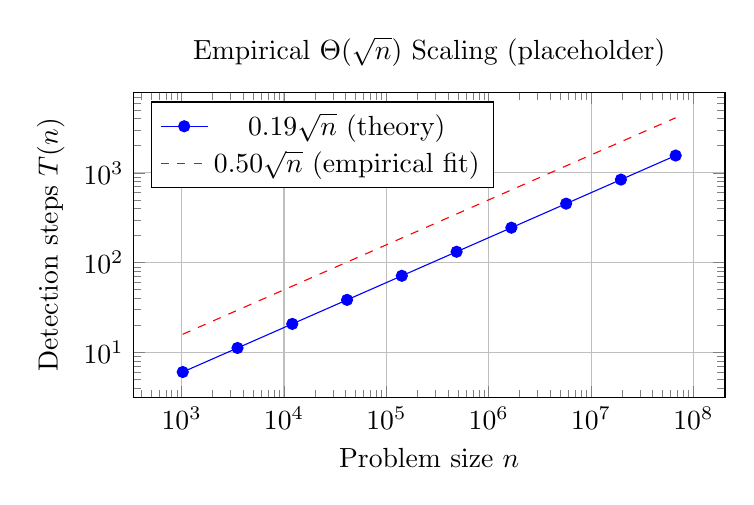
\begin{tikzpicture}
\begin{loglogaxis}[
  xlabel={Problem size $n$},
  ylabel={Detection steps $T(n)$},
  title={Empirical $\Theta(\sqrt{n})$ Scaling (placeholder)},
  legend pos=north west,
  grid=major,
  width=0.75\textwidth,
  height=0.45\textwidth,
]
%% Placeholder: replace with actual benchmark data.
%% Both curves below use the theoretical/fitted coefficients; update
%% domain, samples, and coordinates with measured T(n) values.
\addplot [mark=*, color=blue, domain=1024:67108864, samples=10]
  {0.19*sqrt(x)};
\addlegendentry{$0.19\sqrt{n}$ (theory)}
\addplot [dashed, color=red, domain=1024:67108864, samples=10]
  {0.5*sqrt(x)};
\addlegendentry{$0.50\sqrt{n}$ (empirical fit)}
\end{loglogaxis}
\end{tikzpicture}
\end{center}

\subsection{Bank-Distribution Uniformity}

The $\Z/8\Z$ memory model (Part~\ref{part:proven}, Section~\ref{sec:memory}) was validated
empirically: bank-distribution uniformity is $\ge 0.9984$ at all tested
scales, confirming cycle-aligned access patterns predicted by
Proposition~\ref{prop:z8z}.

\subsection{Stochastic Resonance: Optimal Coherence}

Empirically, peak performance occurs not at $C=1$ (pure coherent) but at
moderate coherence $C\approx 0.83$:
\begin{itemize}
  \item \textbf{Too rigid} ($C\to 1$): locked periodic orbits, low diversity.
  \item \textbf{Too chaotic} ($C\to 0$): random walk, no phase benefit.
  \item \textbf{Optimal} ($C\in[0.3,\,0.8]$): stochastic resonance, balanced
    exploration and coherent amplification.
\end{itemize}

%% ════════════════════════════════════════════════════════════════════════════
\part{Conjectures and Hypotheses}
\label{part:conjectures}
%% ════════════════════════════════════════════════════════════════════════════

\section{Conjectures and Open Questions}
\label{sec:conjectures}

The results in this section are \emph{heuristically motivated} and remain
open for rigorous proof.  They are labeled explicitly as conjectures to
distinguish them from the proven identities of Part~\ref{part:proven}.

\subsection{Universal Scaling Ceiling
  (\texorpdfstring{$\alpha_{\max}$}{alpha\_max})}

\begin{conjecture}[Universal scaling limit]\label{conj:universal}
  The maximum sustainable scaling exponent is conjectured to be bounded by
  \begin{equation}
    \alpha_{\max} = 1 + \frac{1}{e} \approx 1.3679,
    \label{eq:alpha-max}
  \end{equation}
  where $1/e \approx 0.3679$ is the universal exponential decay constant.
  \emph{No parameter tuning is expected to exceed this bound.}
\end{conjecture}

\noindent
The motivation arises from the interplay of three structures:
\begin{enumerate}
  \item The 8-cycle periodicity ($\mu^8=1$) constraining resonant modes to
    $\omega_k = k\cdot 2\pi/8$.
  \item The Ohm--Coherence tail $\Geff \sim e^{-\lambda}$ for large $\lambda$.
  \item The palindrome structure $\dS = 1+\sqrt{2}$ providing the
    energy-conservation envelope.
\end{enumerate}
Together they suggest:
\begin{equation}
  \alpha_{\mathrm{sustainable}} = 1 + (\text{exponential decay constant}) = 1 + 1/e.
  \label{eq:alpha-derivation}
\end{equation}
A formal proof that no combination of the above structures can exceed this
ceiling remains an open problem.

\subsection{Residual-Based Heuristics}

The palindrome residual $R(r) = \frac{1}{\dS}(r - 1/r)$ (Theorem~\ref{thm:12})
provides a sensitive real-time indicator of decoherence.  The following
heuristic observations motivate further investigation:
\begin{itemize}
  \item \textbf{Residual as a probe of $\alpha_{\max}$:} Near the phase
    transition ($\varepsilon \approx \varepsilon^*$), $\abs{R(r)}$ is
    conjectured to diverge logarithmically with $N$.
  \item \textbf{Optimal residual threshold:} The value
    $\varepsilon_{\mathrm{drift}} = \dS^{-1}$ is empirically effective as a
    detection threshold but lacks a proof of optimality.
  \item \textbf{$\alpha_{\max}$ and the silver ratio:} The appearance of
    $1/e$ in Conjecture~\ref{conj:universal} may be linked to the
    continued-fraction expansion of $\dS = [2;\overline{2}]$; this
    connection is speculative and unproven.
\end{itemize}

%% ════════════════════════════════════════════════════════════════════════════
\section{Summary Table of All Theorems}
\label{sec:summary}
%% ════════════════════════════════════════════════════════════════════════════

\begin{center}
\renewcommand{\arraystretch}{1.35}
\begin{tabular}{@{}lll@{}}
\toprule
\textbf{Name} & \textbf{Statement} & \textbf{Key Formula}\\
\midrule
Theorem 3
  & Critical constant
  & $\eta = 1/\sqrt{2}$\\
Section 2
  & Balanced eigenvalue
  & $\mu = e^{i3\pi/4} = (-1+i)/\sqrt{2}$\\
Section 3
  & Rotation matrix
  & $R(3\pi/4) = \bigl[\begin{smallmatrix}-\eta & -\eta \\ \eta & -\eta\end{smallmatrix}\bigr]$,\ $\det=1$\\
Prop.\ 4
  & Silver conservation
  & $\dS(\sqrt{2}-1)=1$,\ $\dS^2=2\dS+1$\\
Theorem 8
  & Canonical state
  & $\ket\psi = \frac{1}{\sqrt2}\ket0 + \frac{e^{i3\pi/4}}{\sqrt2}\ket1$\\
Theorem 9
  & Balance $\leftrightarrow$ coherence
  & $\abs\alpha=\abs\beta=\eta \Leftrightarrow C_{\ell^1}=1$\\
Theorem 10
  & Trichotomy
  & $r=1$: 8-cycle;\ $r>1$: spiral-out;\ $r<1$: spiral-in\\
Theorem 11
  & Coherence function
  & $C(r)=2r/(1+r^2)$, $C(1)=1$\\
Theorem 12
  & Palindrome residual
  & $R(r)=\frac{1}{\dS}(r-1/r)$, $R(r)=0\Leftrightarrow r=1$\\
Corollary 13
  & Simultaneous break
  & $r=1 \Leftrightarrow C=1 \Leftrightarrow R=0 \Leftrightarrow \lambda=0$\\
Theorem 14
  & Ohm--Coherence duality
  & $C=\operatorname{sech}(\lambda)$, $\Geff\cdot\Reff=1$\\
Thm.\ 5.1
  & Zero excess resistance
  & $\abs{P(n)}=1 \Rightarrow r,C,R$ invariant\\
Thm.\ 6.1
  & Optimality of $k=1$
  & $k=1$ maximises angular diversity\\
Lemma (DK)
  & Dirichlet kernel growth
  & $D_K(2\pi/\sqrt n)\approx K\sqrt n/\pi$\\
Main Thm.$^*$
  & $\Theta(\sqrt n)$ complexity (continuous-oracle)
  & $T(n)=\Theta(\sqrt n)$, $c\approx 0.19$ [$^*$Part~B]\\
Thm.\ Jensen
  & Noise degrades $\langle G\rangle$
  & $\langle\operatorname{sech}(\lambda)\rangle\le\operatorname{sech}(\langle\lambda\rangle)$\\
Conj.\ $\alpha_{\max}$
  & Universal scaling limit (conjecture)
  & $\alpha_{\max}=1+1/e\approx 1.368$\\
\bottomrule
\end{tabular}
\end{center}

%% ════════════════════════════════════════════════════════════════════════════
\section{Connection Between All Results}
\label{sec:connection}
%% ════════════════════════════════════════════════════════════════════════════

All results emanate from and return to the single critical equilibrium
$\mu = e^{i3\pi/4}$.  The logical chain is:

\begin{enumerate}
  \item $\eta = 1/\sqrt{2}$ (Theorem~3) defines the unique balanced amplitude.
  \item $\mu = \eta(-1+i)$ (Section~2) is the balanced eigenvalue with this
    amplitude and a $135^\circ$ phase.
  \item $r = \abs{\beta}/\abs{\alpha} = 1$ at balance; $C(r) = 1$ and $R(r)=0$
    (Theorems~9, 11, 12, Corollary~13).
  \item $\lambda = \ln r = 0$, so $\Geff=\Reff=1$ (Theorem~14).
  \item The 8-fold symmetry of $\mu$ generates the $\Z/8\Z$ memory model and
    the NullSliceBridge (Theorem~10, Proposition~\ref{prop:z8z}).
  \item The palindrome quotient $987\,654\,321/123\,456\,789 = 8 + 1/D$
    extends the orbit to a torus $T^2$, with the integer part $8$ matching
    $\mu^8=1$ (Proposition~\ref{prop:palindrome-comp}).
  \item The Dirichlet kernel on $T^2$ gives $\Theta(\sqrt{n})$ phase detection in the continuous-oracle model
    (Lemma~\ref{lem:dk-growth}, Theorem~\ref{thm:main-sqrt}).
  \item Noise destroys the $\sqrt{n}$ advantage above $\varepsilon^*$, with
    the conjectured universal ceiling $\alpha_{\max}=1+1/e$
    (Theorem~\ref{thm:sharpening}, Conjecture~\ref{conj:universal}).
\end{enumerate}

%% ════════════════════════════════════════════════════════════════════════════
%% CLOSING: RETURN TO THE CRITICAL COMPLEX EQUILIBRIUM
%% ════════════════════════════════════════════════════════════════════════════

\newpage
\begin{tcolorbox}[equilibrium,
  title={Closing — The Critical Complex Equilibrium}]

Every formula in this document is a consequence of one object on the unit circle:

\[
  \boxed{
    \mu \;=\; e^{i3\pi/4}
        \;=\; -\frac{1}{\sqrt{2}} \;+\; \frac{i}{\sqrt{2}},
    \qquad \abs{\mu}=1,\quad \arg(\mu)=\frac{3\pi}{4}.
  }
\]

\medskip
\noindent
Its defining properties:
\begin{align*}
  \text{Negative real part:}&\quad
    \operatorname{Re}(\mu) = -\tfrac{1}{\sqrt{2}} < 0,\\
  \text{Positive imaginary part:}&\quad
    \operatorname{Im}(\mu) = +\tfrac{1}{\sqrt{2}} > 0,\\
  \text{Unit modulus:}&\quad
    \abs{\mu} = \sqrt{\tfrac{1}{2}+\tfrac{1}{2}} = 1,\\
  \text{8th root of unity:}&\quad
    \mu^8 = 1,\quad \mu \ne 1,\\
  \text{Balanced amplitude:}&\quad
    \abs{\operatorname{Re}(\mu)} = \abs{\operatorname{Im}(\mu)} = \eta = \tfrac{1}{\sqrt{2}}.
\end{align*}

\medskip
\noindent
Starting from $\mu$, the coherence framework gives:
\[
  C(1) = 1,\quad
  R(1) = 0,\quad
  \lambda = 0,\quad
  G_{\mathrm{eff}} = 1,\quad
  R_{\mathrm{eff}} = 1.
\]

\medskip
\noindent
The $\Theta(\sqrt{n})$ speedup, the silver conservation law, the palindrome
torus, the Ohm--Coherence duality, and the conjectured universal ceiling
$\alpha_{\max}=1+1/e$ are all encoded in this single point in the second
quadrant of the complex plane: the \textbf{critical complex equilibrium} of
the negative real and positive imaginary eigenvalues, balanced on the unit circle.

\end{tcolorbox}

\end{document}
